{\bf The normative theory of \textcite{mattarPrioritizedMemoryAccess2018} suggests that hippocampal replay is a neural substrate for model-based planning. According to the theory, replay is an optimised mechanism by which information from a generative model of the world trains a model-free or reactive decision policy during offline behavioural states \parencite{suttonDynaIntegratedArchitecture1991,moorePrioritizedSweepingReinforcement1993}. This couples the  speed of (online) model-free control with the statistical efficiency and flexibility of (offline) model-based control. However, \textcite{mattarPrioritizedMemoryAccess2018}'s analysis  applies when the model is known, whereas the main challenge of reinforcement learning problems is to learn what to do in the face of ignorance about the model \parencite{kaelblingPlanningActingPartially1998, duffOptimalLearning2002}. Such ignorance requires a delicate balance of exploration and exploitation when making choices. Here, we examine how replay might play a role in a form of approximately optimal exploration. We extend the theory of \textcite{mattarPrioritizedMemoryAccess2018} and derive testable predictions for the patterns of exploratory replay choices one should expect, using a paradigmatic spatial navigation task as an example. Our predictions show the importance of sequence replay, and thus license a range of new experimental paradigms that should further our understanding of offline processing.}

\textcite{mattarPrioritizedMemoryAccess2018} consider replay as the offline activation of remembered or simulated experiences that provide  additional training to  model-free values learnt online. Each individual replay experience updates  the model-free estimate of the long-run value of performing an action  at a state in the task.  Since these model-free action values determine the subject's choices, each replay update can thus improve online behaviour. \textcite{mattarPrioritizedMemoryAccess2018} show that the choice of replay  state and action (which could be distal \parencite{guptaHippocampalReplayNot2010}) that  maximizes the improvement that the subject can expect is determined by two factors: Gain and Need.

The Gain of a replay update is the  local improvement in value  expected for the change in policy engendered by the update.  This quantifies the extra reward the subject expects to receive from the newly changed policy at the update location. By contrast, Need is a global measure of the relevance of the update state (the strength of the successor representation there \parencite{dayanImprovingGeneralizationTemporal1993}) under the old policy. Thus, if Need is low at the potential update state, then the estimated priority for all updates at that state will be low, since the subject does not expect to visit the update state often, and so would not benefit greatly in the long run from that policy update.   

Replay in \textcite{mattarPrioritizedMemoryAccess2018} allows information about reward to be propagated efficiently along sequences of actions that are known to lead to it. This form of model inversion helps a subject  become  proficient at exploiting its knowledge. However, subjects are typically at least partially ignorant about their environments,  because of incomplete initial information, forgetting or unsignalled changes. Sufficient exploration is thus required to gain  new knowledge that can be exploited (Fig~\ref{fig:fig1}); although the benefits of exploration have to be balanced against the costs of not exploiting existing knowledge. The original rationale of the DYNA algorithm \parencite{suttonDynaIntegratedArchitecture1991} that helped inspire \textcite{mattarPrioritizedMemoryAccess2018} was that offline computations could arrange for exploration. Here, we study how replay can play this role.

\begin{figure}[h!]
    \centering
    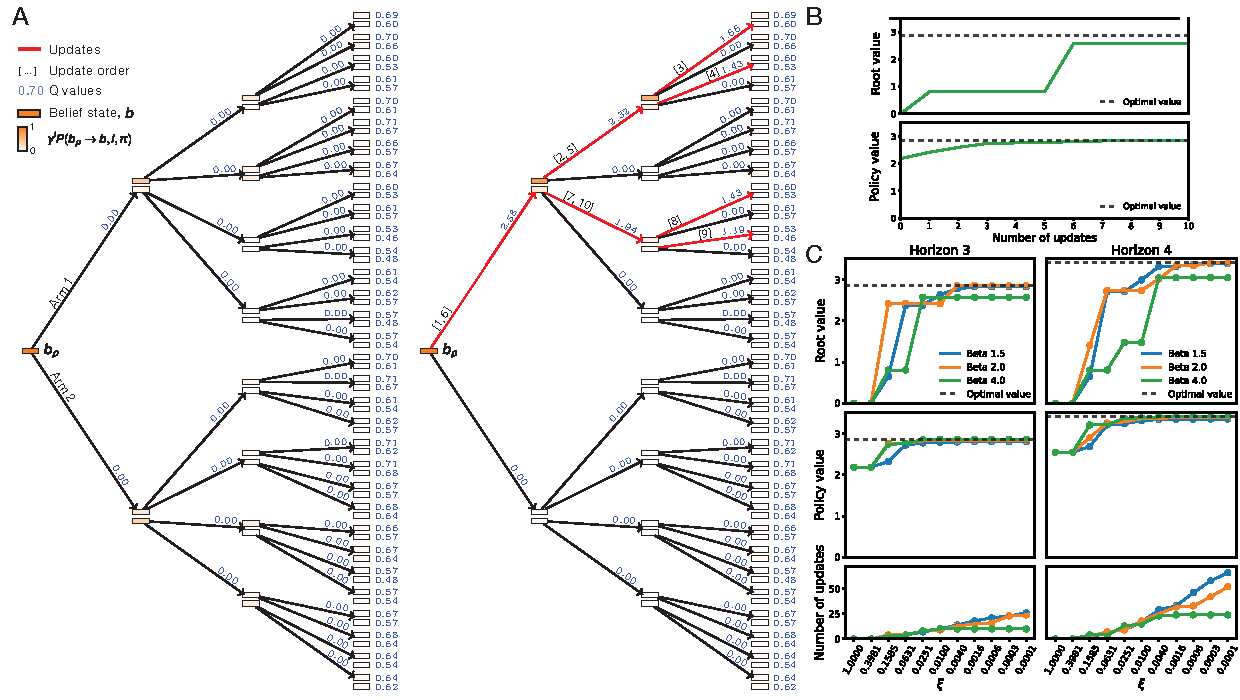
\includegraphics[width=1\textwidth]{Figures/fig1.png}
    \caption{\footnotesize \textbf{Exploitative replay can result in suboptimal behaviour.} A) Normalised state occupancy of the subject during first 2000 moves of exploration and learning in the environment. The start state is located at the bottom and the goal state is shown with the yellow clover. Note that all states were visited by the subject, including those besides the barriers (shown with opaque blue lines). B) Normalised maximal Gain that the subject estimated for the replay of each action (depicted with triangles), averaged across all 2000 moves. We only show actions for which the Gain was estimated to be positive. The actions which the subject would replay yielded a more exploitative policy which helped the subject acquire reward at a higher rate. C) Normalised maximal Need for each state that the subject estimated, also averaged over those same 2000 moves. All values were additionally averaged over 10 simulations. D-F) Same as (A-C) but for additional 2000 moves during which the top barrier was removed. Note that the estimated Gain did not change. Moreover, the state occupancy profile in D), as well as the estimated Need in F) highlight how the subject's behaviour reduced to pure exploitation. Because of the environmental change, however, this behaviour was rendered suboptimal due to the existence of a shorter path  that the subject  did not discover.}
    \label{fig:fig1}
\end{figure}

There are two coarse flavours of exploration: undirected and directed \parencite{wilsonBalancingExplorationExploitation2021}, along with many heuristic and approximate versions of the latter. Undirected exploration comes from introducing stochasticity into choice. Although sometimes effective \parencite{dawCorticalSubstratesExploratory2006}, it is typically suboptimal. Rather, exploration should be directed to reducing the uncertainty about which actions in the environment are ultimately best \parencite{feldbaumDualControlTheory1965}.  One standard heuristic \parencite{suttonDynaIntegratedArchitecture1991} (see also \parencite{agrawalTemporalDynamicsOpportunity2020}) is to add a form of notional exploration bonus to the outcome of  actions whose consequences are uncertain.\cut{, which assumes that uncertainty grows with the time since the action was last attempted, and makes the exploration bonus follow suit (see also \parencite{agrawalTemporalDynamicsOpportunity2020}). }

Optimal exploration generates  bonuses by maintaining probabilistically-correct beliefs about the environment and accounting 
carefully for the immediate and longer term consequences of resolving the implied uncertainty  \parencite{gittinsBanditProcessesDynamic1979,duffQLearningBanditProblems1995}. This amounts to performing regular optimal control, but in what is known as a belief-state decision problem in which the physical state of the subject in the environment is augmented by the subject's beliefs about the environment (in our later spatial case, how likely it thinks barriers are to have been removed). Such careful accounting is radically computationally intractable, for instance because the space of all possible beliefs is continuous, implying that the optimal policy can be very complex. We show how exploratory forms of Gain and Need can generalize the use of replay to realize a limited version of this accounting offline.

Most studies of hippocampal replay  have  focused on  navigation tasks. We therefore sought to make testable predictions for exploratory replay in a rich spatial environment inspired by \textcite{tolmanCognitiveMapsRats1948} 
(and report in the supplement similar results on the simpler, theoretically more tractable, case of multi-arm bandit problems). Our maze comprises three corridors which merge onto the common stem leading to the goal location (Fig~\ref{fig:fig1}). Those corridors differ in length, and thus an optimal reward-maximising agent (and rats \parencite{tolmanCognitiveMapsRats1948}) would prefer the shortest corridor. However, either just the shortest, or all but the longest, path might possibly be blocked by barriers. The accompanying uncertainty provides the motivation for exploration. 

\begin{figure}[h!]
    \centering
    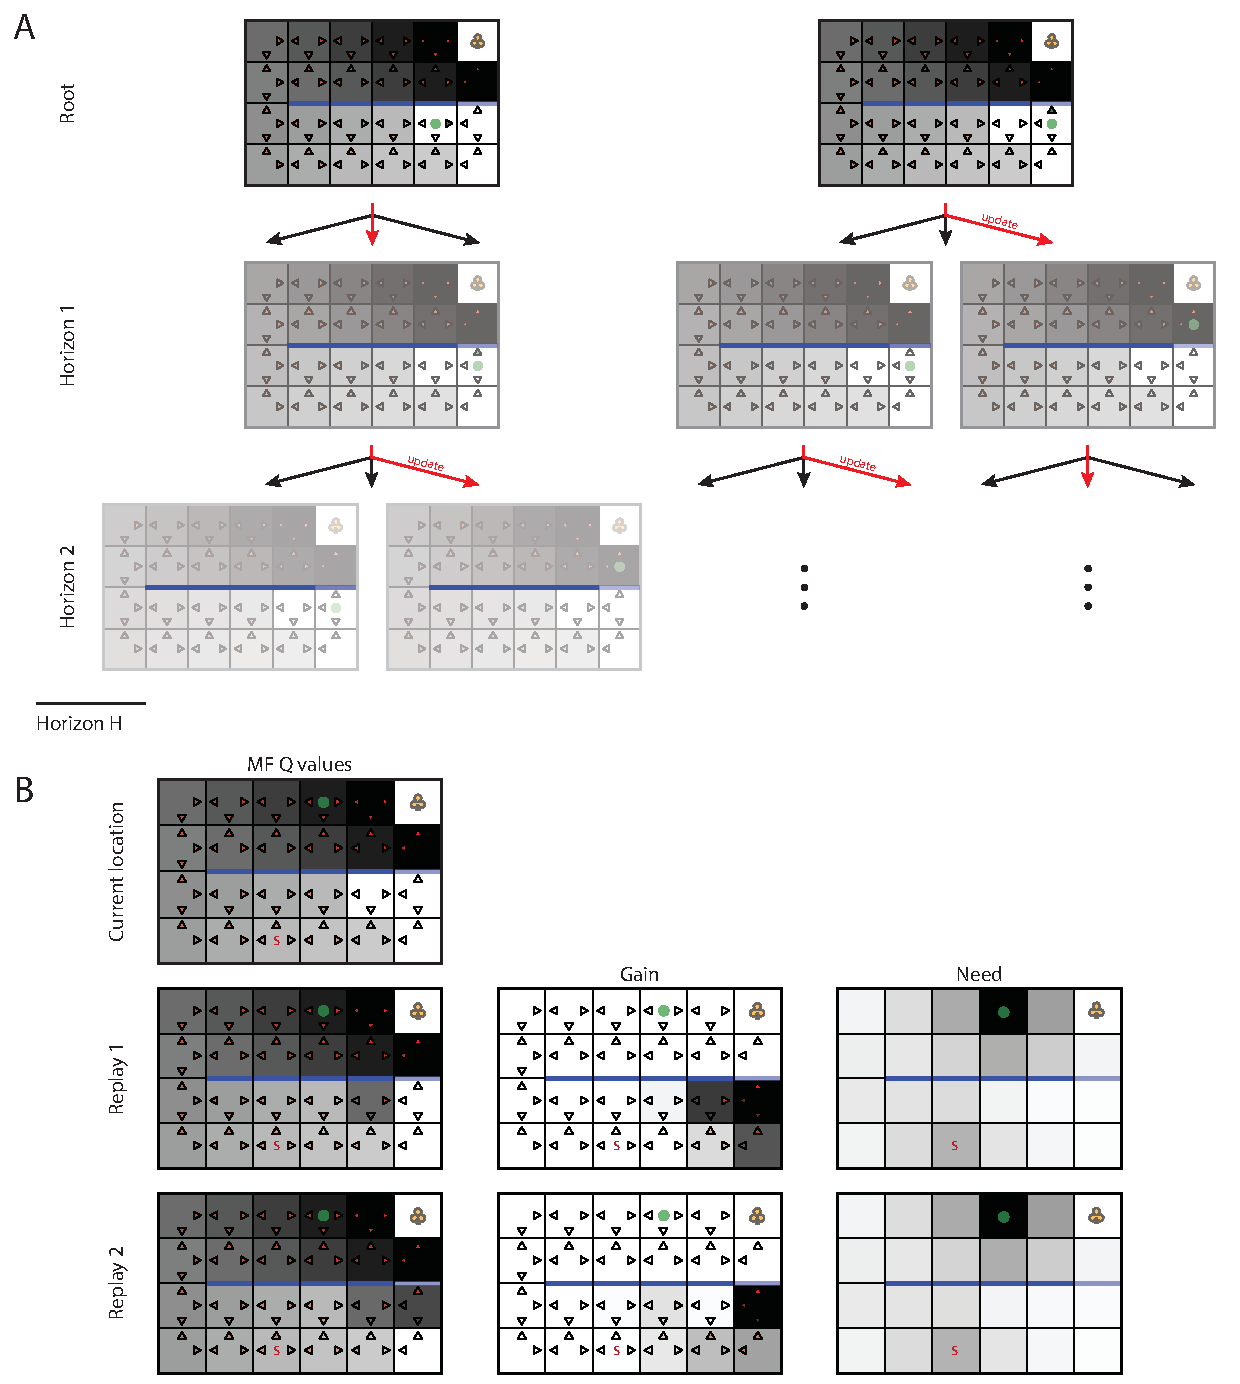
\includegraphics[width=1\textwidth]{Figures/fig2.png}
    \caption{\footnotesize \textbf{Exploratory replay leads to online discoveries, but potentially inadequate promulgation.} A) Prior state of knowledge of the subject. The intensity of the colour of each action arrow shows the respective model-free $Q$-values. Collectively, the action values represent the subject's model-free behavioural policy (i.e., the subject is more likely to choose actions with higher estimated $Q$-values -- those are highlighted with yellow outlines). Similarly, the states are coloured according to the maximal model-free $Q$-value at each state (which corresponds to state values). The inset next to the top barrier indicates the subject's prior belief about its presence (for the other barrier, the subject was certain that the path was blocked). The red dotted line shows the expected probability that the barrier is absent. The subject itself (green dot) is located at the start state. The goal state with reward is denoted with the yellow clover. B) Changes in the subject's model-free policy occasioned by exploratory replay updates. The numbers next to each action arrow indicate the order in which the replay updates were executed. C) New model-free policy which resulted from exploratory replay updates in B). Note how the action values now indicate that the subject should go towards the upper barrier. D) After pursuing the exploratory policy, the subject attempted to cross the top barrier; unfortunately, the barrier was found to be present -- this is indicated by both the subject's model-free $Q$-value associated with that action which was learnt online, as well as its new belief. E-F) Same as in B-C) but after the online discovery of the present barrier in D). The first replay choice of the subject correctly propagated the negative value of the present barrier to the immediately preceding state. However, as opposed to propagating this information deeper towards the start state, and hence correcting the exploratory policy in the light of the new information, the next replay choice of the subject made it more likely to visit an adjacent state which still contained the previously propagated exploration bonus, and hence had an erroneously (given the subject's new knowledge) high value.}
    \label{fig:fig2}
\end{figure}

For exploratory Gain: suppose that the subject is at a physical location just next to a barrier and is contemplating the action that might cross over and get close to the goal. To the extent the agent is uncertain that the barrier is 
absent, the action will fail, leading  to the belief that the barrier is there, and no Gain. However, as much as the agent is uncertain that the barrier is present, this action will succeed, leaving the subject in a new location, and with a new belief that the barrier is absent. This imagined outcome is associated with high Gain, because of the
implied shortcut estimated, in our account, based on the high model-free values for the new location. 

However, exploratory Need suffers from a chicken-and-egg problem in that if the          
subject adopts the purely exploitative policy of the known-to-be-open           
longest path, then the Need for the potential shortcut transition is            
zero (as the state next to the barrier is not visited). For simplicity, we make the approximation of including  stochasticity in the subject's behavioural policy (for instance, in the form of undirected exploration) such that Need is strictly positive for all possible belief states. This is achieved through applying a softmax behavioural policy \parencite{dawCorticalSubstratesExploratory2006}. 

The calculations of exploratory Gain and Need differ crucially from \textcite{mattarPrioritizedMemoryAccess2018} in terms of generalization. Individual physical locations (such as those next to barriers) can be visited with different beliefs about the environment. Importantly, discovering that a barrier is present/absent is information for all belief states associated with that barrier. This requires the subject to generalise the benefit of potential discoveries across multiple belief states.

As mentioned earlier, optimally accounting for the evolution of the subject's beliefs is woefully intractable. We therefore incorporated a form of second-order certainty equivalence approximation \parencite{dayanExplorationBonusesDual1996} for the estimation of exploratory Need. The subject optimally tracks how its belief will evolve up to a limited planning horizon beyond which the residual uncertainty remains fixed. This means that the subject still maintains its subjective uncertainty about the possible futures (unlike  conventional forms of certainty equivalence \parencite{cozzolinoMarkovianDecisionProcesses1965}); however, it assumes that no new knowledge can be acquired or environmental changes take place beyond its planning horizon.

We simulated behaviour in the Tolman maze and examined the replay patterns  produced as a result of  uncertainty about the presence of the upper barrier (Fig~\ref{fig:fig2}). Note that the subject has to choose which arm to pursue at a decision point remote from the potential barrier location. There is thus substantial cost for exploration: the subject
has to have sufficient belief that the barrier is open  -- otherwise the potential benefit of exploration (discovering a shortcut) would not exceed the cost of deviating from the current behavioural policy (current reward rate) \parencite{nivTonicDopamineOpportunity2007}.

\begin{figure}[h!]
    \centering
    \includegraphics[width=1\textwidth]{Figures/fig3.png}
    \caption{\footnotesize \textbf{Sequence replay helps deep value propagation.} The layout of the figure is the same as in Fig~\ref{fig:fig2}. A-C) Show the subject's initial and uncertain state of knowledge, changes to the online behavioural policy occasioned by exploratory replay, and the new updated exploratory policy due to such replay, respectively. The crucial difference being that the replay in B) was \cut{backward arrows along the green line} a sequence event -- i.e., the whole chain of actions was updated simultaneously (the actions which were updated in the replayed sequence are linked by a green line). D-F) Again, the subject discovered the top barrier, learnt about its presence online and engaged in replay to recompile its model-free behavioural policy in the light of the negative information. Note how, in this case, sequence replay in E) resulted in deep propagation of the value of such information all the way towards the start state. The sequence replay thus enabled the subject to  correct its exploratory policy appropriately.}
    \label{fig:fig3}
\end{figure}

Here, the subject's uncertainty resulted in consecutive replay updates which originated at the potential barrier location and progressed towards the subject's location in a reverse manner (Fig~\ref{fig:fig2}A-C). Those replays propagated the value of exploring the barrier towards the subject's current location, and the resulting new model-free behavioural policy indicated exploration was worthwhile (Fig~\ref{fig:fig2}C). As just discussed, the extent to which the subject was uncertain determined how large was the exploratory bonus that reached the subject's current state -- and thus produced policies with different incentives for exploration \toga{should fig S5 have single-action replay updates instead? since we only talk about sequence replay later}(Figs~\ref{fig:supp5} and~\ref{fig:supp6}). 

Resolving uncertainty can often result in unfortunate outcomes, for instance if the barrier is found actually to be present (Fig~\ref{fig:fig2}D). If this happens, it is important for the subject to  correct the full exploratory policy that had led to the discovery in the light of the negative information it acquired. We find that in our simulated Tolman maze, single-action replay updates do not handle this appropriately: the discovered value of the present barrier does not propagate deeply enough towards those states which had been updated with the exploratory bonus of the obsolete belief (Fig~\ref{fig:fig2}E-F). This is because  single-action updates are myopic: the estimated benefit of a single-action update does not account for how that update can affect the benefit of potential future updates. This problem does not arise if the shortcut is found to be available, since then the subject can efficiently exploit its new policy.

One plausible solution is to consider the benefit of simultaneously updating a sequence of actions, as opposed to  relying solely on updates at single states. This benefit combines Gain, that accumulates with the propagated policy changes (provided that all those changes result in policy improvements), as well as Need along that sequence of actions. We found that sequence replay results in deep propagation of the value of a discovered barrier, along the whole chain of actions which had previously been endowed with the exploration bonus (Fig~\ref{fig:fig3}).

Experimental evidence implicates the hippocampus in constructing replay sequences through previously unexplored spaces \parencite{guptaHippocampalReplayNot2010, olafsdottirHippocampalPlaceCells2015}. In our account, this corresponds to replay in potential future belief states which the subject has not visited yet but imagines to encounter. We manipulated the barrier configuration in our maze to produce a corridor segment in the central arm with both sides occluded by barriers (Fig~\ref{fig:fig4}). Examining the replay patterns chosen by the subject due to its uncertainty about the presence of both barriers revealed sequence replay in the corridor. Such replay propagated the exploratory value of learning about the possibility of entering the corridor (resolving uncertainty about the bottom barrier), exiting it (learning about the top barrier) and ending up in a state close to the goal.

\begin{figure}[h!]
    \centering
    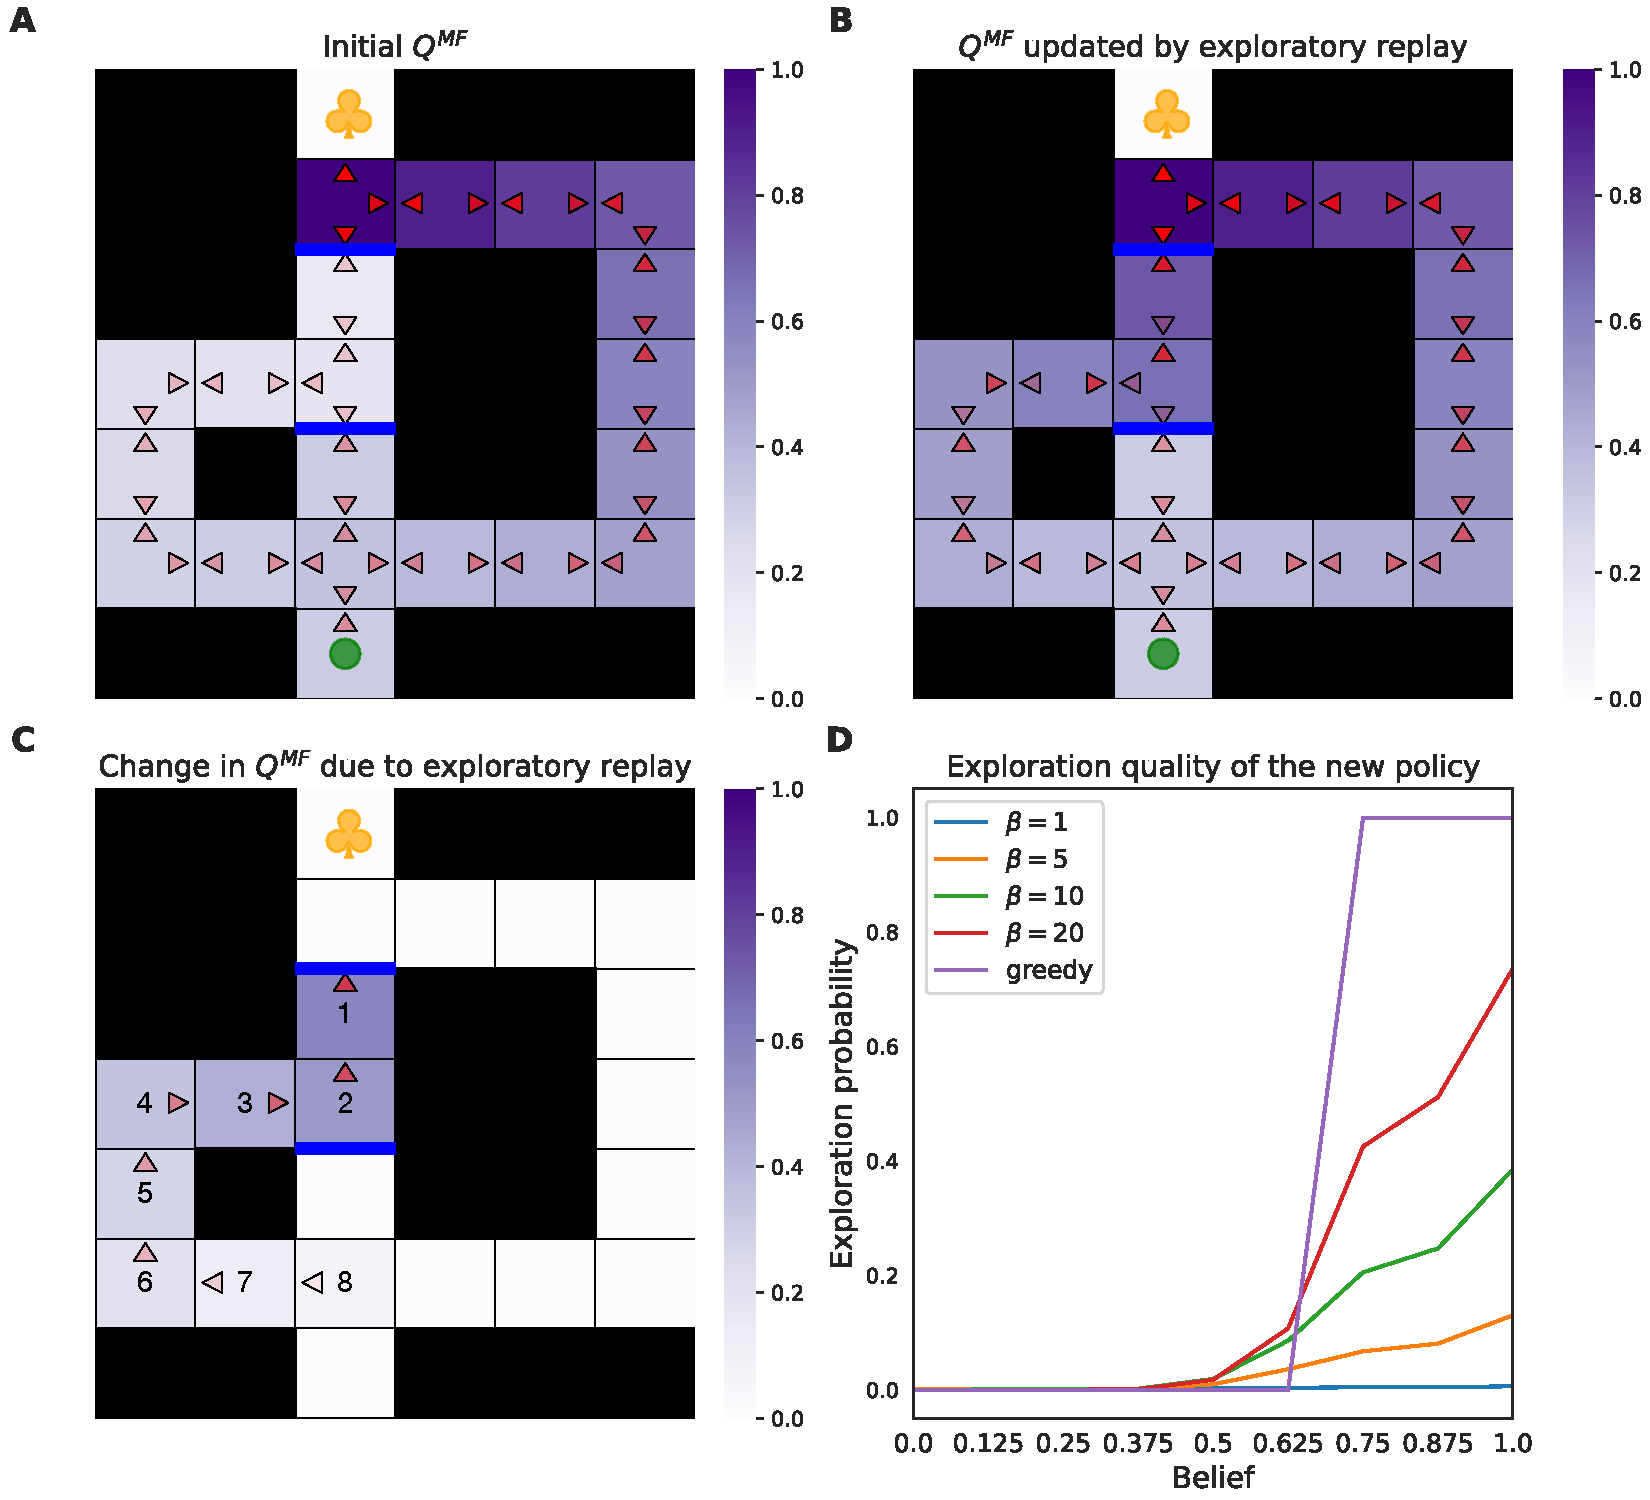
\includegraphics[width=1\textwidth]{Figures/fig4.png}
    \caption{\footnotesize \textbf{Replay in a blocked corridor.} A) Initial state of knowledge of the subject. Note that the model-free $Q$-values in the blocked corridor are all initialised to $0$, thus mimicking the subject's inexperience with the segment. The subject's belief state comprises its uncertainty about the presence of the top and bottom barriers that create the corridor. B) Replay choices of the subject due to its initial and uncertain state of knowledge. Note that replays inside the corridor correspond to a different belief state since they follow the potential transition through the bottom barrier which the subject has to first learn about. C) New exploratory policy occasioned by the replay updates in B).}
    \label{fig:fig4}
\end{figure}

Some of the most important facets of learning in the brain involve building inverse models: this characterizes bottom-up, recognition, models of sensory processing in cortex; the maintenance and expansion of the relationship between cortical and hippocampal representations in memory; and the determination of policies that maximize reward and minimize punishment given information about the environment. Offline processing, evident in replay, offers a way of building and refining inverse models of all these forms without disturbing ongoing behaviour. However, to determine good policies, it is not enough to build an inverse model based on just current information; active observers have the obligation to collect new information too, and balance this against exploitation. This obligation can be satisfied by inverting a more sophisticated model of the environment that includes uncertainty; here, we showed how to conceive of (reverse) replay as performing this inverse. This provided new insights into the nature and structure of offline activity -- for instance surfacing the importance of sequence replay, as well as predictions for new experimental paradigms.

